\documentclass[14pt]{extbook}
\usepackage{multicol, enumerate, enumitem, hyperref, color, soul, setspace, parskip, fancyhdr} %General Packages
\usepackage{amssymb, amsthm, amsmath, bbm, latexsym, units, mathtools} %Math Packages
\everymath{\displaystyle} %All math in Display Style
% Packages with additional options
\usepackage[headsep=0.5cm,headheight=12pt, left=1 in,right= 1 in,top= 1 in,bottom= 1 in]{geometry}
\usepackage[usenames,dvipsnames]{xcolor}
\usepackage{dashrule}  % Package to use the command below to create lines between items
\newcommand{\litem}[1]{\item#1\hspace*{-1cm}\rule{\textwidth}{0.4pt}}
\pagestyle{fancy}
\lhead{Progress Quiz 4}
\chead{}
\rhead{Version A}
\lfoot{9187-5854}
\cfoot{}
\rfoot{Spring 2021}
\begin{document}

\begin{enumerate}
\litem{
Determine the domain of the function below.\[ f(x) = \frac{4}{20x^{2} -9 x -20} \]\begin{enumerate}[label=\Alph*.]
\item \( \text{All Real numbers except } x = a \text{ and } x = b, \text{ where } a \in [-22, -15] \text{ and } b \in [17, 21] \)
\item \( \text{All Real numbers except } x = a, \text{ where } a \in [-22, -15] \)
\item \( \text{All Real numbers except } x = a, \text{ where } a \in [-0.8, 0.2] \)
\item \( \text{All Real numbers except } x = a \text{ and } x = b, \text{ where } a \in [-0.8, 0.2] \text{ and } b \in [1.25, 2.25] \)
\item \( \text{All Real numbers.} \)

\end{enumerate} }
\litem{
Choose the equation of the function graphed below.
\begin{center}
    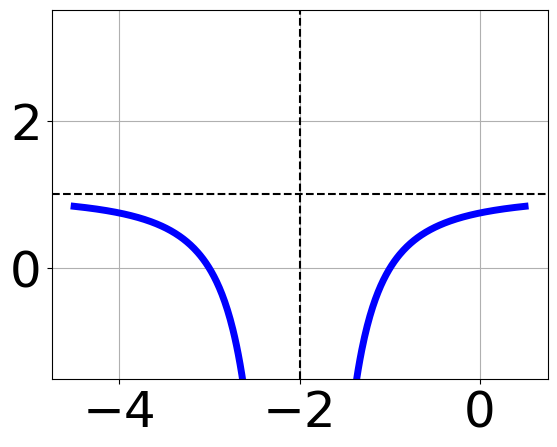
\includegraphics[width=0.5\textwidth]{../Figures/rationalGraphToEquationCopyA.png}
\end{center}
\begin{enumerate}[label=\Alph*.]
\item \( f(x) = \frac{1}{x - 2} + 7 \)
\item \( f(x) = \frac{1}{(x - 2)^2} + 7 \)
\item \( f(x) = \frac{-1}{x + 2} + 7 \)
\item \( f(x) = \frac{-1}{(x + 2)^2} + 7 \)
\item \( \text{None of the above} \)

\end{enumerate} }
\litem{
Solve the rational equation below. Then, choose the interval(s) that the solution(s) belongs to.\[ \frac{-4}{9x -4} + 7 = \frac{-6}{72x -32} \]\begin{enumerate}[label=\Alph*.]
\item \( x \in [0.5,2.5] \)
\item \( x \in [-0.42,-0.29] \)
\item \( x_1 \in [-0.42, -0.29] \text{ and } x_2 \in [-0.5,1.5] \)
\item \( \text{All solutions lead to invalid or complex values in the equation.} \)
\item \( x_1 \in [0.41, 0.48] \text{ and } x_2 \in [-0.5,1.5] \)

\end{enumerate} }
\litem{
Determine the domain of the function below.\[ f(x) = \frac{4}{18x^{2} +18 x -36} \]\begin{enumerate}[label=\Alph*.]
\item \( \text{All Real numbers except } x = a \text{ and } x = b, \text{ where } a \in [-19, -16] \text{ and } b \in [33, 38] \)
\item \( \text{All Real numbers.} \)
\item \( \text{All Real numbers except } x = a \text{ and } x = b, \text{ where } a \in [-4, -1] \text{ and } b \in [0, 4] \)
\item \( \text{All Real numbers except } x = a, \text{ where } a \in [-4, -1] \)
\item \( \text{All Real numbers except } x = a, \text{ where } a \in [-19, -16] \)

\end{enumerate} }
\litem{
Choose the graph of the equation below.\[ f(x) = \frac{1}{x - 1} + 3 \]\begin{enumerate}[label=\Alph*.]
\begin{multicols}{2}\item 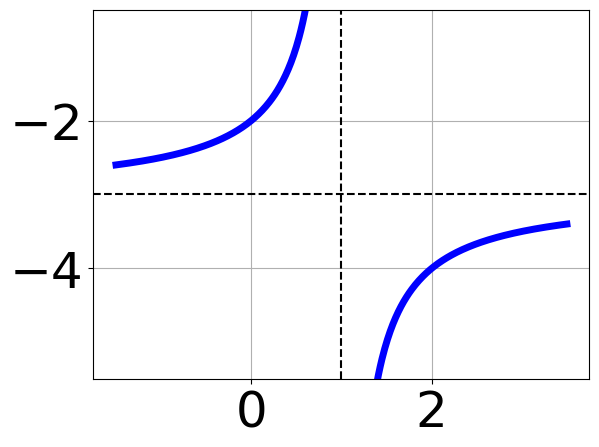
\includegraphics[width = 0.3\textwidth]{../Figures/rationalEquationToGraphCopyAA.png}\item 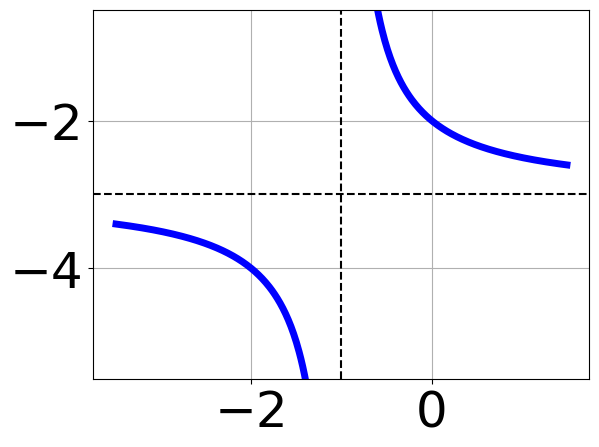
\includegraphics[width = 0.3\textwidth]{../Figures/rationalEquationToGraphCopyBA.png}\item 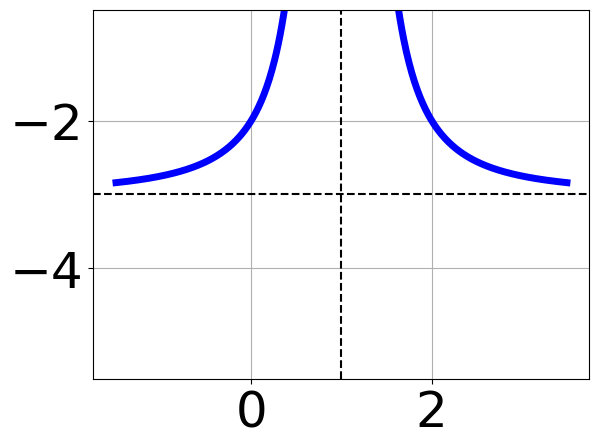
\includegraphics[width = 0.3\textwidth]{../Figures/rationalEquationToGraphCopyCA.png}\item 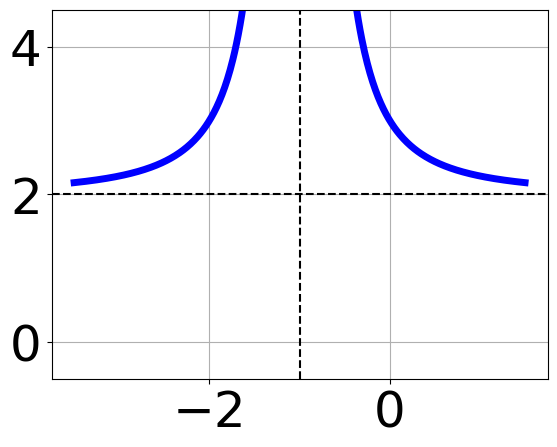
\includegraphics[width = 0.3\textwidth]{../Figures/rationalEquationToGraphCopyDA.png}\end{multicols}\item None of the above.
\end{enumerate} }
\litem{
Solve the rational equation below. Then, choose the interval(s) that the solution(s) belongs to.\[ \frac{56}{28x + 56} + 1 = \frac{56}{28x + 56} \]\begin{enumerate}[label=\Alph*.]
\item \( \text{All solutions lead to invalid or complex values in the equation.} \)
\item \( x_1 \in [-3, 1] \text{ and } x_2 \in [-2,-1] \)
\item \( x \in [-3.0,-1.0] \)
\item \( x_1 \in [-3, 1] \text{ and } x_2 \in [1,6] \)
\item \( x \in [2,4] \)

\end{enumerate} }
\litem{
Solve the rational equation below. Then, choose the interval(s) that the solution(s) belongs to.\[ \frac{6x}{4x -6} + \frac{-4x^{2}}{28x^{2} -58 x + 24} = \frac{-5}{7x -4} \]\begin{enumerate}[label=\Alph*.]
\item \( \text{All solutions lead to invalid or complex values in the equation.} \)
\item \( x_1 \in [-1.15, 0.02] \text{ and } x_2 \in [0.91,1.23] \)
\item \( x \in [0.93,1.79] \)
\item \( x \in [0.54,0.72] \)
\item \( x_1 \in [-1.15, 0.02] \text{ and } x_2 \in [1.09,1.6] \)

\end{enumerate} }
\litem{
Choose the equation of the function graphed below.
\begin{center}
    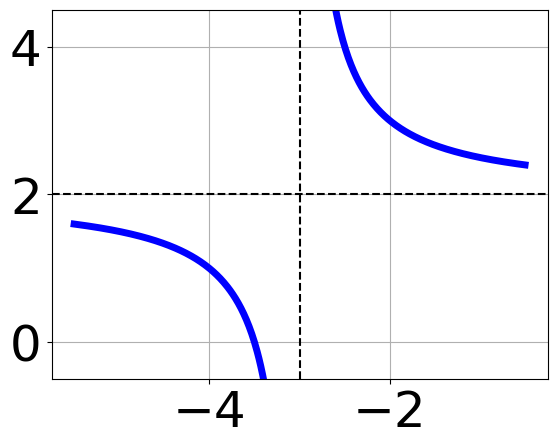
\includegraphics[width=0.5\textwidth]{../Figures/rationalGraphToEquationA.png}
\end{center}
\begin{enumerate}[label=\Alph*.]
\item \( f(x) = \frac{1}{x + 1} - 1 \)
\item \( f(x) = \frac{-1}{x - 1} - 1 \)
\item \( f(x) = \frac{-1}{(x - 1)^2} - 1 \)
\item \( f(x) = \frac{1}{(x + 1)^2} - 1 \)
\item \( \text{None of the above} \)

\end{enumerate} }
\litem{
Choose the graph of the equation below.\[ f(x) = \frac{-1}{x - 1} + 2 \]\begin{enumerate}[label=\Alph*.]
\begin{multicols}{2}\item 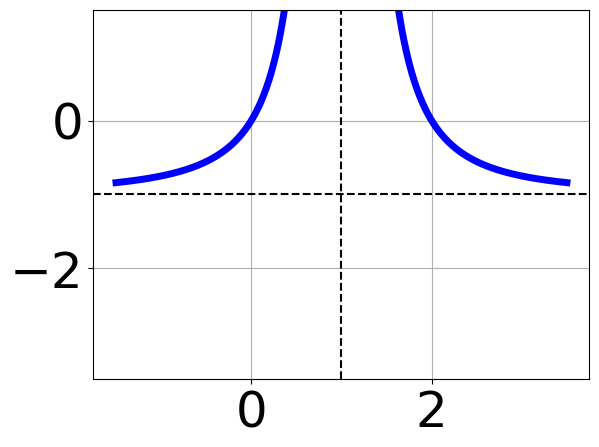
\includegraphics[width = 0.3\textwidth]{../Figures/rationalEquationToGraphAA.png}\item 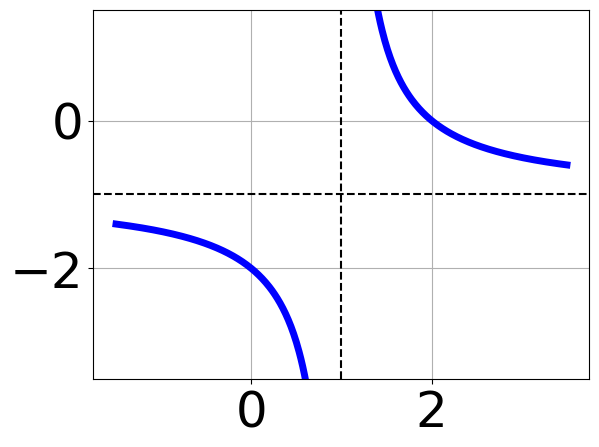
\includegraphics[width = 0.3\textwidth]{../Figures/rationalEquationToGraphBA.png}\item 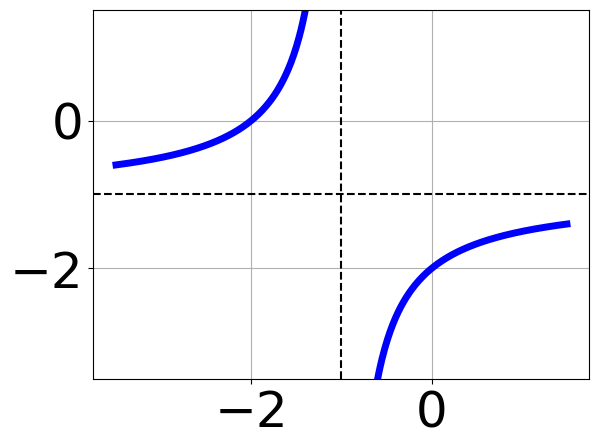
\includegraphics[width = 0.3\textwidth]{../Figures/rationalEquationToGraphCA.png}\item 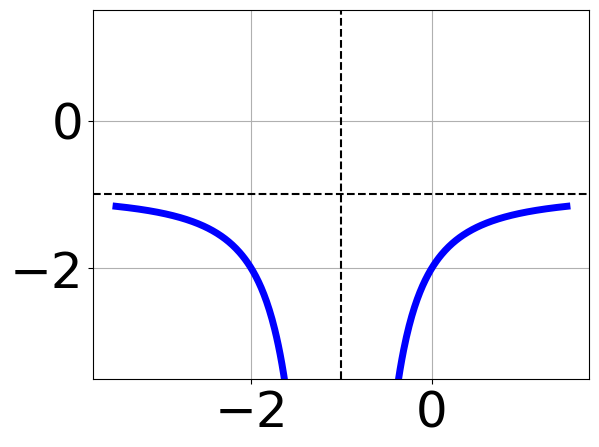
\includegraphics[width = 0.3\textwidth]{../Figures/rationalEquationToGraphDA.png}\end{multicols}\item None of the above.
\end{enumerate} }
\litem{
Solve the rational equation below. Then, choose the interval(s) that the solution(s) belongs to.\[ \frac{5x}{-2x -5} + \frac{-4x^{2}}{-6x^{2} -x + 35} = \frac{3}{3x -7} \]\begin{enumerate}[label=\Alph*.]
\item \( x \in [2.16,2.42] \)
\item \( x_1 \in [0.44, 1.31] \text{ and } x_2 \in [-3.2,-1.4] \)
\item \( \text{All solutions lead to invalid or complex values in the equation.} \)
\item \( x \in [0.76,2.18] \)
\item \( x_1 \in [0.44, 1.31] \text{ and } x_2 \in [-0.6,2.8] \)

\end{enumerate} }
\end{enumerate}

\end{document}